\documentclass{standalone}
\usepackage{tikz}
\usetikzlibrary{patterns, positioning}
\usepackage[sfdefault]{ClearSans} %% option 'sfdefault' activates Clear Sans as the default text font
\usepackage[T1]{fontenc}

\begin{document}
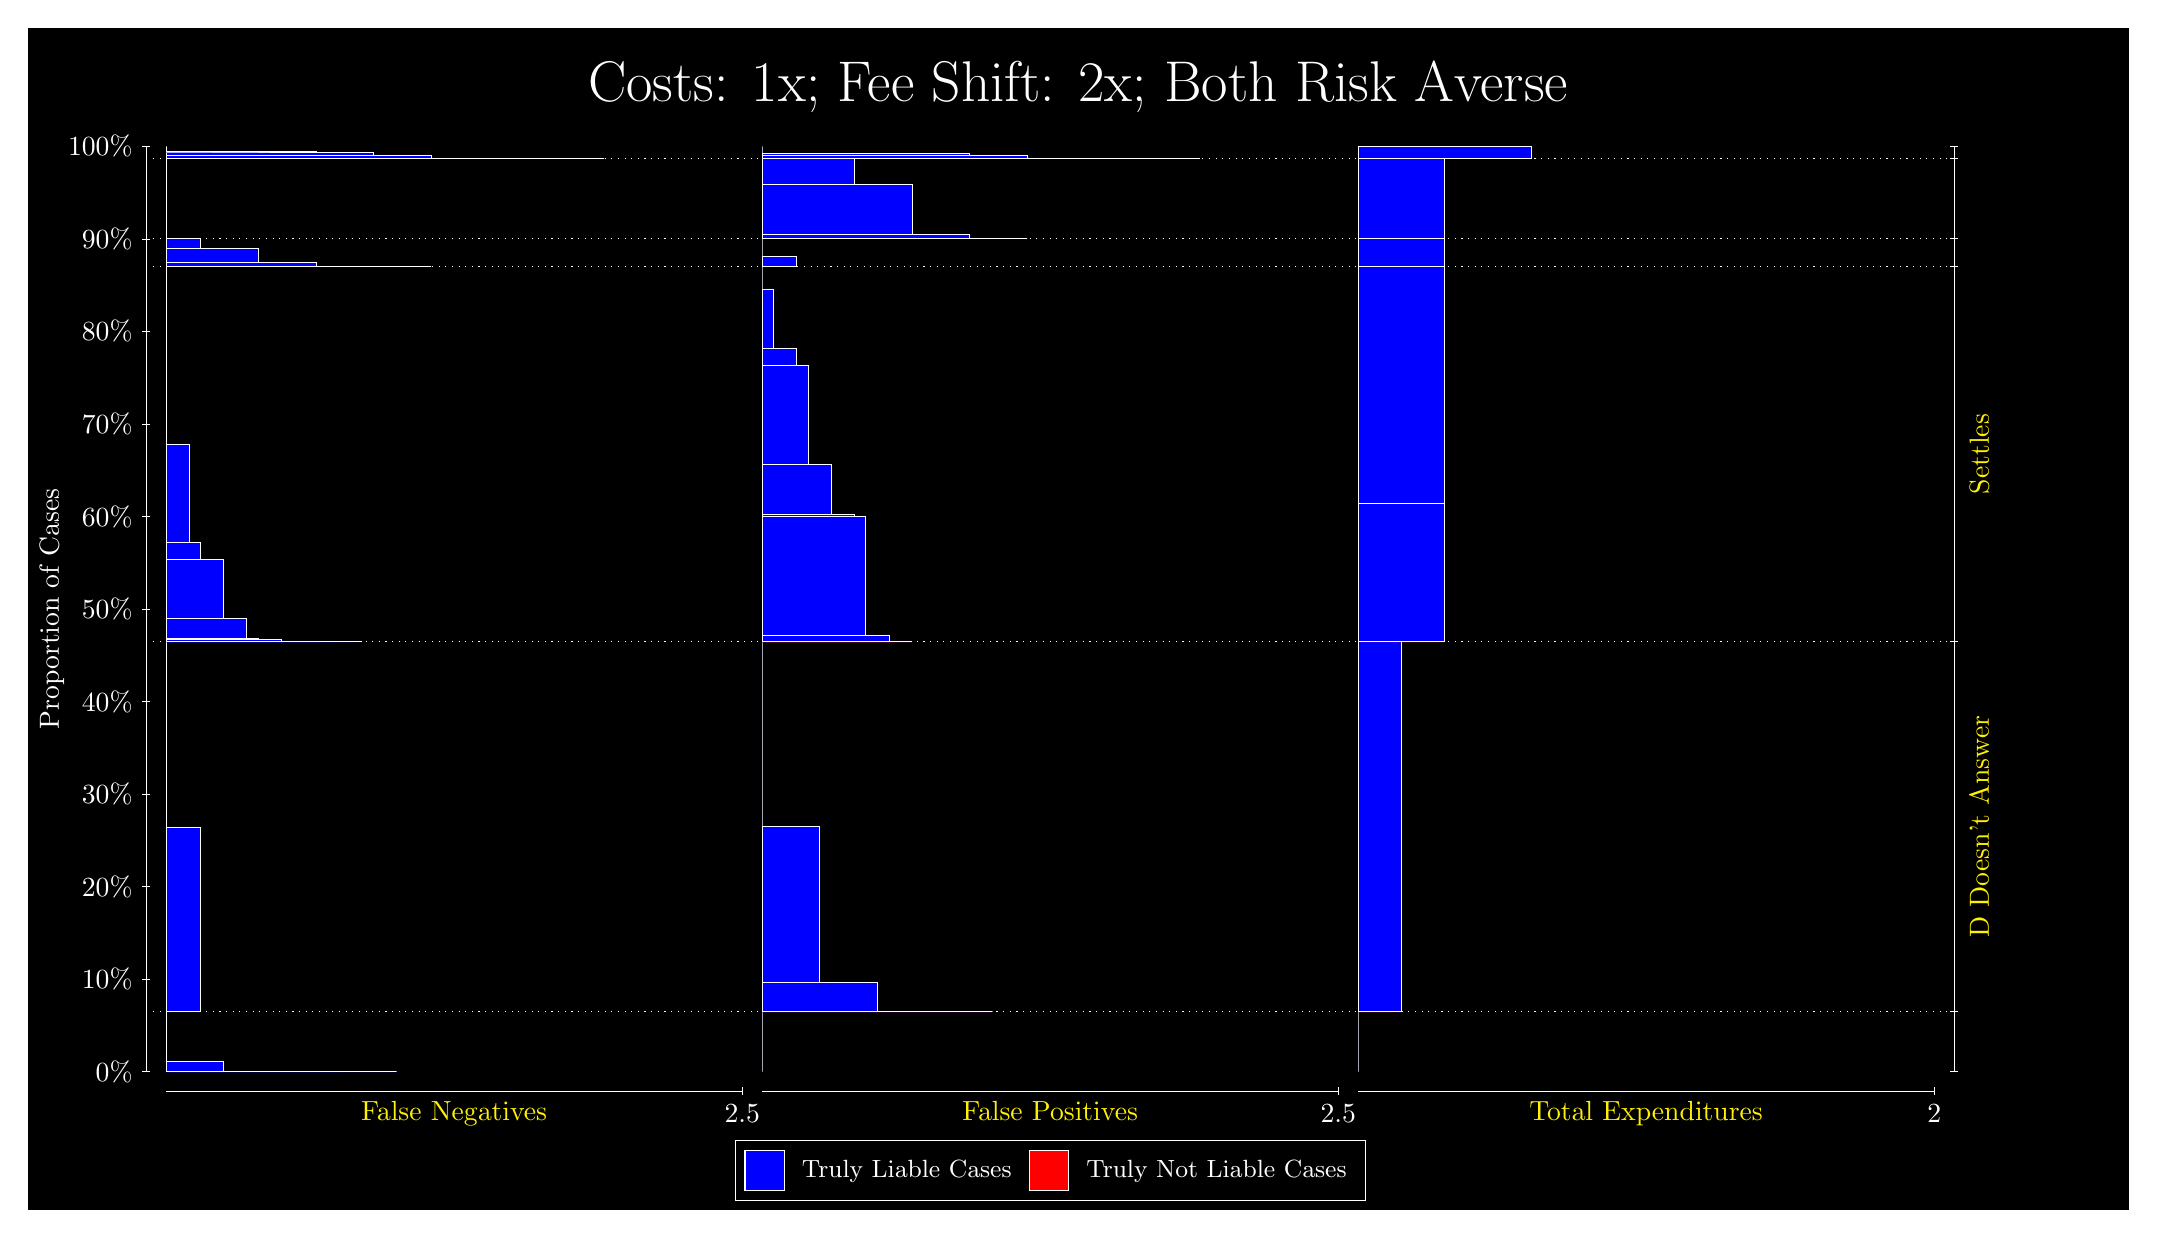
\begin{tikzpicture}
\draw[fill=black] (0,0) rectangle (26.667,15);
\draw[text=white] (0,13.5) rectangle (26.667,15) node[midway] {\huge Costs: 1x; Fee Shift: 2x; Both Risk Averse};
\draw[white, very thin] (1.5,1.75) -- (1.5,13.5);
\node[rotate=90, text=white, anchor=center] at (0.3, 7.625) {Proportion of Cases};
\draw[white, very thin] (1.45,1.75) -- (1.55,1.75);
\node[text=white, anchor=east] at (1.45, 1.75) {0\%};
\draw[white, very thin] (1.45,2.925) -- (1.55,2.925);
\node[text=white, anchor=east] at (1.45, 2.925) {10\%};
\draw[white, very thin] (1.45,4.1) -- (1.55,4.1);
\node[text=white, anchor=east] at (1.45, 4.1) {20\%};
\draw[white, very thin] (1.45,5.275) -- (1.55,5.275);
\node[text=white, anchor=east] at (1.45, 5.275) {30\%};
\draw[white, very thin] (1.45,6.45) -- (1.55,6.45);
\node[text=white, anchor=east] at (1.45, 6.45) {40\%};
\draw[white, very thin] (1.45,7.625) -- (1.55,7.625);
\node[text=white, anchor=east] at (1.45, 7.625) {50\%};
\draw[white, very thin] (1.45,8.8) -- (1.55,8.8);
\node[text=white, anchor=east] at (1.45, 8.8) {60\%};
\draw[white, very thin] (1.45,9.975) -- (1.55,9.975);
\node[text=white, anchor=east] at (1.45, 9.975) {70\%};
\draw[white, very thin] (1.45,11.15) -- (1.55,11.15);
\node[text=white, anchor=east] at (1.45, 11.15) {80\%};
\draw[white, very thin] (1.45,12.325) -- (1.55,12.325);
\node[text=white, anchor=east] at (1.45, 12.325) {90\%};
\draw[white, very thin] (1.45,13.5) -- (1.55,13.5);
\node[text=white, anchor=east] at (1.45, 13.5) {100\%};

\draw[white, very thin] (24.457,1.75) -- (24.457,13.5);
\draw[white, very thin] (24.407,1.75) -- (24.507,1.75);
\node[anchor=west] at (24.407, 1.75) {};
\draw[white, very thin] (24.407,2.5101) -- (24.507,2.5101);
\node[anchor=west] at (24.407, 2.5101) {};
\draw[white, very thin] (24.407,7.2086) -- (24.507,7.2086);
\node[anchor=west] at (24.407, 7.2086) {};
\draw[white, very thin] (24.407,11.975) -- (24.507,11.975);
\node[anchor=west] at (24.407, 11.975) {};
\draw[white, very thin] (24.407,12.331) -- (24.507,12.331);
\node[anchor=west] at (24.407, 12.331) {};
\draw[white, very thin] (24.407,13.351) -- (24.507,13.351);
\node[anchor=west] at (24.407, 13.351) {};
\draw[white, very thin] (24.407,13.5) -- (24.507,13.5);
\node[anchor=west] at (24.407, 13.5) {};

\draw[white, very thin, fill=blue] (1.75,1.75) rectangle (4.6775,1.75);
\draw[white, very thin, fill=blue] (1.75,1.75) rectangle (3.9457,1.75);
\draw[white, very thin, fill=blue] (1.75,1.75) rectangle (3.2138,1.7511);
\draw[white, very thin, fill=blue] (1.75,1.7511) rectangle (2.4819,1.8745);
\draw[white, very thin, fill=red] (1.75,1.8745) rectangle (1.75,1.8745);
\draw[white, very thin, fill=blue] (1.75,1.8745) rectangle (1.75,2.5101);
\draw[white, very thin, fill=blue] (1.75,2.5101) rectangle (2.1891,4.8562);
\draw[white, very thin, fill=red] (1.75,4.8562) rectangle (1.75,4.8562);
\draw[white, very thin, fill=blue] (1.75,4.8562) rectangle (1.75,7.2086);
\draw[white, very thin, fill=blue] (1.75,7.2086) rectangle (4.2384,7.2086);
\draw[white, very thin, fill=blue] (1.75,7.2086) rectangle (3.9457,7.2086);
\draw[white, very thin, fill=blue] (1.75,7.2086) rectangle (3.6529,7.2086);
\draw[white, very thin, fill=blue] (1.75,7.2086) rectangle (3.5065,7.2132);
\draw[white, very thin, fill=blue] (1.75,7.2132) rectangle (3.2138,7.2395);
\draw[white, very thin, fill=blue] (1.75,7.2395) rectangle (2.921,7.2503);
\draw[white, very thin, fill=blue] (1.75,7.2503) rectangle (2.7746,7.5004);
\draw[white, very thin, fill=blue] (1.75,7.5004) rectangle (2.4819,8.2515);
\draw[white, very thin, fill=blue] (1.75,8.2515) rectangle (2.1891,8.4682);
\draw[white, very thin, fill=blue] (1.75,8.4682) rectangle (2.0428,9.7196);
\draw[white, very thin, fill=red] (1.75,9.7196) rectangle (1.75,9.7196);
\draw[white, very thin, fill=blue] (1.75,9.7196) rectangle (1.75,11.975);
\draw[white, very thin, fill=blue] (1.75,11.975) rectangle (5.1167,11.975);
\draw[white, very thin, fill=blue] (1.75,11.975) rectangle (4.3848,11.976);
\draw[white, very thin, fill=blue] (1.75,11.976) rectangle (3.6529,12.025);
\draw[white, very thin, fill=blue] (1.75,12.025) rectangle (2.921,12.208);
\draw[white, very thin, fill=blue] (1.75,12.208) rectangle (2.1891,12.331);
\draw[white, very thin, fill=red] (1.75,12.331) rectangle (1.75,12.331);
\draw[white, very thin, fill=blue] (1.75,12.331) rectangle (2.1891,12.335);
\draw[white, very thin, fill=red] (1.75,12.335) rectangle (1.75,12.335);
\draw[white, very thin, fill=blue] (1.75,12.335) rectangle (1.75,13.351);
\draw[white, very thin, fill=blue] (1.75,13.351) rectangle (7.3123,13.351);
\draw[white, very thin, fill=blue] (1.75,13.351) rectangle (6.5805,13.351);
\draw[white, very thin, fill=blue] (1.75,13.351) rectangle (5.8486,13.353);
\draw[white, very thin, fill=blue] (1.75,13.353) rectangle (5.1167,13.385);
\draw[white, very thin, fill=blue] (1.75,13.385) rectangle (4.3848,13.429);
\draw[white, very thin, fill=blue] (1.75,13.429) rectangle (3.6529,13.434);
\draw[white, very thin, fill=blue] (1.75,13.434) rectangle (3.0674,13.434);
\draw[white, very thin, fill=blue] (1.75,13.434) rectangle (2.921,13.434);
\draw[white, very thin, fill=blue] (1.75,13.434) rectangle (2.3355,13.434);
\draw[white, very thin, fill=red] (1.75,13.434) rectangle (1.75,13.434);
\draw[white, very thin, fill=blue] (1.75,13.434) rectangle (1.75,13.5);
\draw[white, very thin, fill=red] (9.3189,1.75) rectangle (9.3189,1.75);
\draw[white, very thin, fill=blue] (9.3189,1.75) rectangle (9.3189,2.5101);
\draw[white, very thin, fill=red] (9.3189,2.5101) rectangle (12.246,2.5101);
\draw[white, very thin, fill=blue] (9.3189,2.5101) rectangle (12.246,2.5101);
\draw[white, very thin, fill=blue] (9.3189,2.5101) rectangle (11.515,2.5131);
\draw[white, very thin, fill=blue] (9.3189,2.5131) rectangle (10.783,2.8858);
\draw[white, very thin, fill=blue] (9.3189,2.8858) rectangle (10.051,4.8624);
\draw[white, very thin, fill=blue] (9.3189,4.8624) rectangle (9.3189,7.2086);
\draw[white, very thin, fill=red] (9.3189,7.2086) rectangle (11.222,7.2086);
\draw[white, very thin, fill=blue] (9.3189,7.2086) rectangle (11.222,7.2086);
\draw[white, very thin, fill=red] (9.3189,7.2086) rectangle (10.929,7.2086);
\draw[white, very thin, fill=blue] (9.3189,7.2086) rectangle (10.929,7.2948);
\draw[white, very thin, fill=red] (9.3189,7.2948) rectangle (10.636,7.2948);
\draw[white, very thin, fill=blue] (9.3189,7.2948) rectangle (10.636,8.7982);
\draw[white, very thin, fill=blue] (9.3189,8.7982) rectangle (10.49,8.8232);
\draw[white, very thin, fill=blue] (9.3189,8.8232) rectangle (10.197,9.4638);
\draw[white, very thin, fill=blue] (9.3189,9.4638) rectangle (9.9044,10.715);
\draw[white, very thin, fill=blue] (9.3189,10.715) rectangle (9.758,10.932);
\draw[white, very thin, fill=blue] (9.3189,10.932) rectangle (9.4652,11.683);
\draw[white, very thin, fill=blue] (9.3189,11.683) rectangle (9.3189,11.975);
\draw[white, very thin, fill=red] (9.3189,11.975) rectangle (9.758,11.975);
\draw[white, very thin, fill=blue] (9.3189,11.975) rectangle (9.758,12.098);
\draw[white, very thin, fill=blue] (9.3189,12.098) rectangle (9.3189,12.331);
\draw[white, very thin, fill=red] (9.3189,12.331) rectangle (12.686,12.331);
\draw[white, very thin, fill=blue] (9.3189,12.331) rectangle (12.686,12.331);
\draw[white, very thin, fill=blue] (9.3189,12.331) rectangle (11.954,12.389);
\draw[white, very thin, fill=blue] (9.3189,12.389) rectangle (11.222,13.018);
\draw[white, very thin, fill=blue] (9.3189,13.018) rectangle (10.49,13.347);
\draw[white, very thin, fill=blue] (9.3189,13.347) rectangle (9.758,13.351);
\draw[white, very thin, fill=red] (9.3189,13.351) rectangle (14.881,13.351);
\draw[white, very thin, fill=blue] (9.3189,13.351) rectangle (14.881,13.351);
\draw[white, very thin, fill=red] (9.3189,13.351) rectangle (14.149,13.351);
\draw[white, very thin, fill=blue] (9.3189,13.351) rectangle (14.149,13.351);
\draw[white, very thin, fill=red] (9.3189,13.351) rectangle (13.417,13.351);
\draw[white, very thin, fill=blue] (9.3189,13.351) rectangle (13.417,13.354);
\draw[white, very thin, fill=red] (9.3189,13.354) rectangle (12.686,13.354);
\draw[white, very thin, fill=blue] (9.3189,13.354) rectangle (12.686,13.385);
\draw[white, very thin, fill=blue] (9.3189,13.385) rectangle (11.954,13.415);
\draw[white, very thin, fill=blue] (9.3189,13.415) rectangle (11.222,13.417);
\draw[white, very thin, fill=blue] (9.3189,13.417) rectangle (10.49,13.417);
\draw[white, very thin, fill=red] (9.3189,13.417) rectangle (9.9044,13.417);
\draw[white, very thin, fill=blue] (9.3189,13.417) rectangle (9.9044,13.417);
\draw[white, very thin, fill=blue] (9.3189,13.417) rectangle (9.758,13.417);
\draw[white, very thin, fill=red] (9.3189,13.417) rectangle (9.3189,13.417);
\draw[white, very thin, fill=blue] (9.3189,13.417) rectangle (9.3189,13.5);
\draw[white, very thin, fill=red] (16.888,1.75) rectangle (16.888,1.75);
\draw[white, very thin, fill=blue] (16.888,1.75) rectangle (16.888,2.5101);
\draw[white, very thin, fill=red] (16.888,2.5101) rectangle (17.437,2.5101);
\draw[white, very thin, fill=blue] (16.888,2.5101) rectangle (17.437,7.2086);
\draw[white, very thin, fill=red] (16.888,7.2086) rectangle (17.986,7.2086);
\draw[white, very thin, fill=blue] (16.888,7.2086) rectangle (17.986,8.9653);
\draw[white, very thin, fill=red] (16.888,8.9653) rectangle (17.986,8.9653);
\draw[white, very thin, fill=blue] (16.888,8.9653) rectangle (17.986,11.975);
\draw[white, very thin, fill=red] (16.888,11.975) rectangle (17.986,11.975);
\draw[white, very thin, fill=blue] (16.888,11.975) rectangle (17.986,12.331);
\draw[white, very thin, fill=red] (16.888,12.331) rectangle (17.986,12.331);
\draw[white, very thin, fill=blue] (16.888,12.331) rectangle (17.986,13.351);
\draw[white, very thin, fill=red] (16.888,13.351) rectangle (19.083,13.351);
\draw[white, very thin, fill=blue] (16.888,13.351) rectangle (19.083,13.5);
\draw[white, dotted] (1.5,2.5101) -- (24.457,2.5101);
\draw[white, dotted] (1.5,7.2086) -- (24.457,7.2086);
\draw[white, dotted] (1.5,11.975) -- (24.457,11.975);
\draw[white, dotted] (1.5,12.331) -- (24.457,12.331);
\draw[white, dotted] (1.5,13.351) -- (24.457,13.351);
\draw[white, very thin] (1.75,1.5) -- (9.0689,1.5);
\node[text=yellow, anchor=north] at (5.4094, 1.5) {False Negatives};
\draw[white, very thin] (9.0689,1.45) -- (9.0689,1.55);
\node[text=white, anchor=north] at (9.0689, 1.45) {2.5};

\draw[white, very thin] (9.3189,1.5) -- (16.638,1.5);
\node[text=yellow, anchor=north] at (12.978, 1.5) {False Positives};
\draw[white, very thin] (16.638,1.45) -- (16.638,1.55);
\node[text=white, anchor=north] at (16.638, 1.45) {2.5};

\draw[white, very thin] (16.888,1.5) -- (24.207,1.5);
\node[text=yellow, anchor=north] at (20.547, 1.5) {Total Expenditures};
\draw[white, very thin] (24.207,1.45) -- (24.207,1.55);
\node[text=white, anchor=north] at (24.207, 1.45) {2};


\node[text=yellow, centered, rotate=90] at (24.777, 4.8593) {D Doesn't Answer};
\node[text=yellow, centered, rotate=90] at (24.777, 9.5917) {Settles};




\draw (12.978300999999998,1.5) node[draw=none] (baseCoordinate) {};
\begin{scope}[align=center]
        \matrix[scale=0.5, draw=white, below=0.5cm of baseCoordinate, nodes={draw}, column sep=0.1cm]{
            \node[rectangle, draw, minimum width=0.5cm, minimum height=0.5cm, fill=blue] {}; &
            \node[draw=none, font=\small, text=white] (B) {Truly Liable Cases}; &
            \node[rectangle, draw, minimum width=0.5cm, minimum height=0.5cm, fill=red] {}; &
            \node[draw=none, font=\small, text=white] (B) {Truly Not Liable Cases}; \\
            };
\end{scope}

\end{tikzpicture}
\end{document}